\section{Iron --- Spin-polarized WFs, DOS, projected WFs versus \MLWFs}
\label{sec8:Iron}

\begin{itemize}
	\item Outline : {\it Generate both maximally-localized and projected Wannier functions for ferromagnetic bcc Fe. Calculate the total and orbital-projected density of states by Wannier interpolation.}
\end{itemize}

\begin{figure}[h!]
\centering
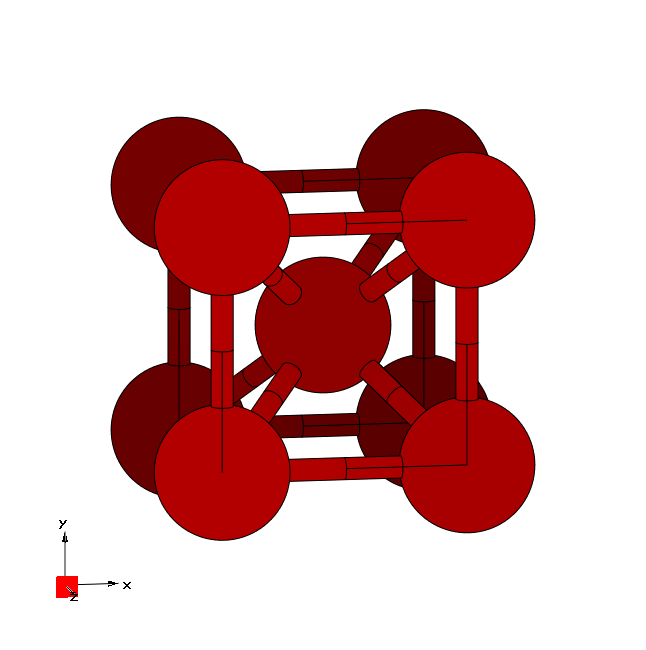
\includegraphics[width=0.25\columnwidth,trim={45pt 45pt 55pt 55pt},clip]{figure/example08/iron.png}
\caption{Unit cell of Iron crystal plotted with the \xcrysden{} program.}
\label{fig8.0}
\end{figure}

\begin{enumerate}
	\item[1-5] {\it Converged values for the total spread functional and its components for both spin channels are shown in Tab.~\ref{tab8.1}.} 
	The final state for spin-up MLWFs is
	\begin{tcolorbox}[sharp corners,boxrule=0.5pt]
	{\small
	\begin{verbatim}
	 Final State
  WF centre and spread    1  (  0.709852,  0.000108,  0.000131 )     1.08935224
  WF centre and spread    2  (  0.000131,  0.000053, -0.709852 )     1.08935218
  WF centre and spread    3  ( -0.709852, -0.000108, -0.000131 )     1.08935221
  WF centre and spread    4  (  0.000108, -0.709852, -0.000053 )     1.08935218
  WF centre and spread    5  ( -0.000131, -0.000053,  0.709852 )     1.08935226
  WF centre and spread    6  (  0.000000,  0.000000,  0.000000 )     0.43234428
  WF centre and spread    7  ( -0.000000,  0.000000,  0.000000 )     0.43234429
  WF centre and spread    8  ( -0.000108,  0.709852,  0.000053 )     1.08935225
  WF centre and spread    9  (  0.000000,  0.000000, -0.000000 )     0.43234428
  Sum of centres and spreads (  0.000000, -0.000000, -0.000000 )     7.83314616
 
         Spreads (Ang^2)       Omega I      =     5.948424630
        ================       Omega D      =     0.017027691
                               Omega OD     =     1.867693841
    Final Spread (Ang^2)       Omega Total  =     7.833146162
 ------------------------------------------------------------------------------
	\end{verbatim}
	}
	\end{tcolorbox}
	and for spin-down MLWFs is
	  \begin{tcolorbox}
  {\small
	\begin{verbatim}[sharp corners,boxrule=0.5pt]
	 Final State
  WF centre and spread    1  ( -0.685467, -0.000123,  0.000259 )     1.10268580
  WF centre and spread    2  ( -0.000259, -0.000207, -0.685467 )     1.10268617
  WF centre and spread    3  (  0.685468,  0.000123, -0.000259 )     1.10268605
  WF centre and spread    4  ( -0.000123,  0.685467, -0.000207 )     1.10268595
  WF centre and spread    5  (  0.000259,  0.000207,  0.685467 )     1.10268552
  WF centre and spread    6  (  0.000000,  0.000000, -0.000000 )     0.41116646
  WF centre and spread    7  ( -0.000000,  0.000000, -0.000000 )     0.41116648
  WF centre and spread    8  (  0.000123, -0.685467,  0.000207 )     1.10268572
  WF centre and spread    9  (  0.000000,  0.000000,  0.000000 )     0.41116644
  Sum of centres and spreads (  0.000000, -0.000000,  0.000000 )     7.84961460
 
         Spreads (Ang^2)       Omega I      =     5.946718376
        ================       Omega D      =     0.014524283
                               Omega OD     =     1.888371944
    Final Spread (Ang^2)       Omega Total  =     7.849614603
 ------------------------------------------------------------------------------
	\end{verbatim}
	}
	\end{tcolorbox}
	As it is clear from the output file snippets above, the $s,p$ and $d$ orbitals hybridize to give rise to two groups of functions for both spin channels. A first group made of 6 MLWFs coming from the hybridisation of $sp^3$ and $d_{e_g}$ MLWFs, with a total spread of 1.089(1.103)\angsqd{} for spin-up(down). A second group made of 3 MLWFs with a $d_{t_{2g}}$ character, with a total spread of 0.432(0.4112)\angsqd{} for spin-up(down). Two sample MLWFs, one for each group, are shown in \Fig{fig8.3}.
	\end{enumerate}

	\begin{figure}[h!]
	\centering
	\subfloat[$sp^3$ + $d_{e_g}$]{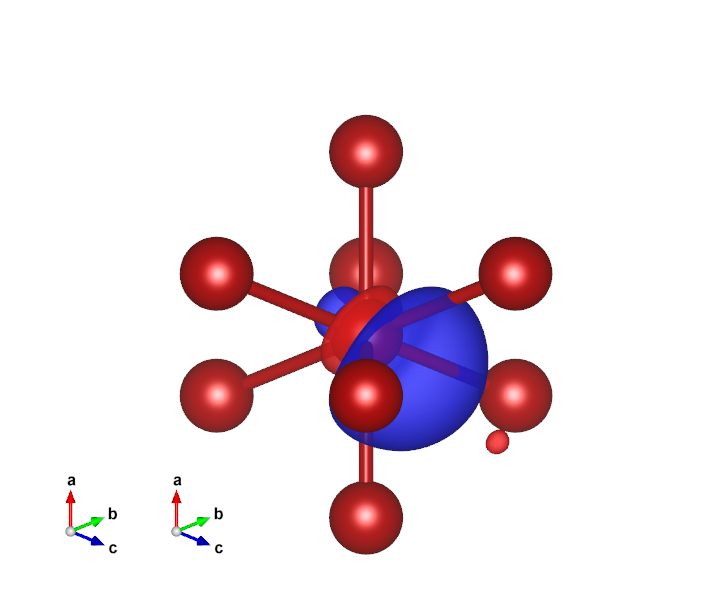
\includegraphics[scale=0.25,trim={150pt 0pt 150pt 70pt},clip]{figure/example08/iron_up_00001.png}}
	\hspace{3cm}
	\centering
	\subfloat[$d_{t_{2g}}$]{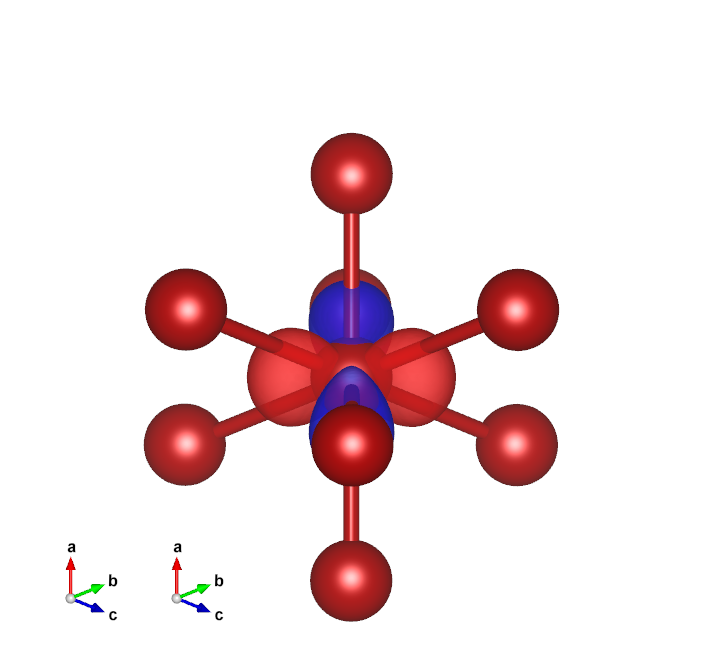
\includegraphics[scale=0.23,trim={140pt 0pt 100pt 70pt},clip]{figure/example08/iron_up_00006.png}}
	\caption{2 representative MLWFs from the wannierisation of 9 spin-up bands of iron. a) A representative of the hybrid ($sp^3$ and $d_{e_g}$) group of MLWFs. b) A representative of the $d_{t_{2g}}$ group of MLWFs.}\label{fig8.3}
	\end{figure}

\begin{table}[t!]
	\centering
	\captionsetup{width=.5\textwidth}
	\caption{Converged values of the components of spread functional and their sums for both spin chanels for ferromagnetic bcc Fe, given in \angsqd{}.}
	\begin{tabular}{@{} llllll @{}}\toprule[1.5pt]
	spin & $\Omega$ & $\Omega\tinysub{I}$ & $\Omega\tinysub{OD}$ & $\Omega\tinysub{D}$ & $N_{\mathrm{iter}}$ \\\midrule
	up & 7.8331 & 5.9484 & 1.8677 & 0.0170 & 400 \\
	down & 7.8496 & 5.9467 & 1.8884 & 0.0145 & 400 \\\bottomrule[1pt]
	\end{tabular}\label{tab8.1}
\end{table} 
	

\subsection*{Density of states}
\begin{itemize}
	\item {\it run {\tt postw90} and plot the DOS with {\tt gnuplot}}
\end{itemize}
	\begin{figure}[h!]
	\centering
	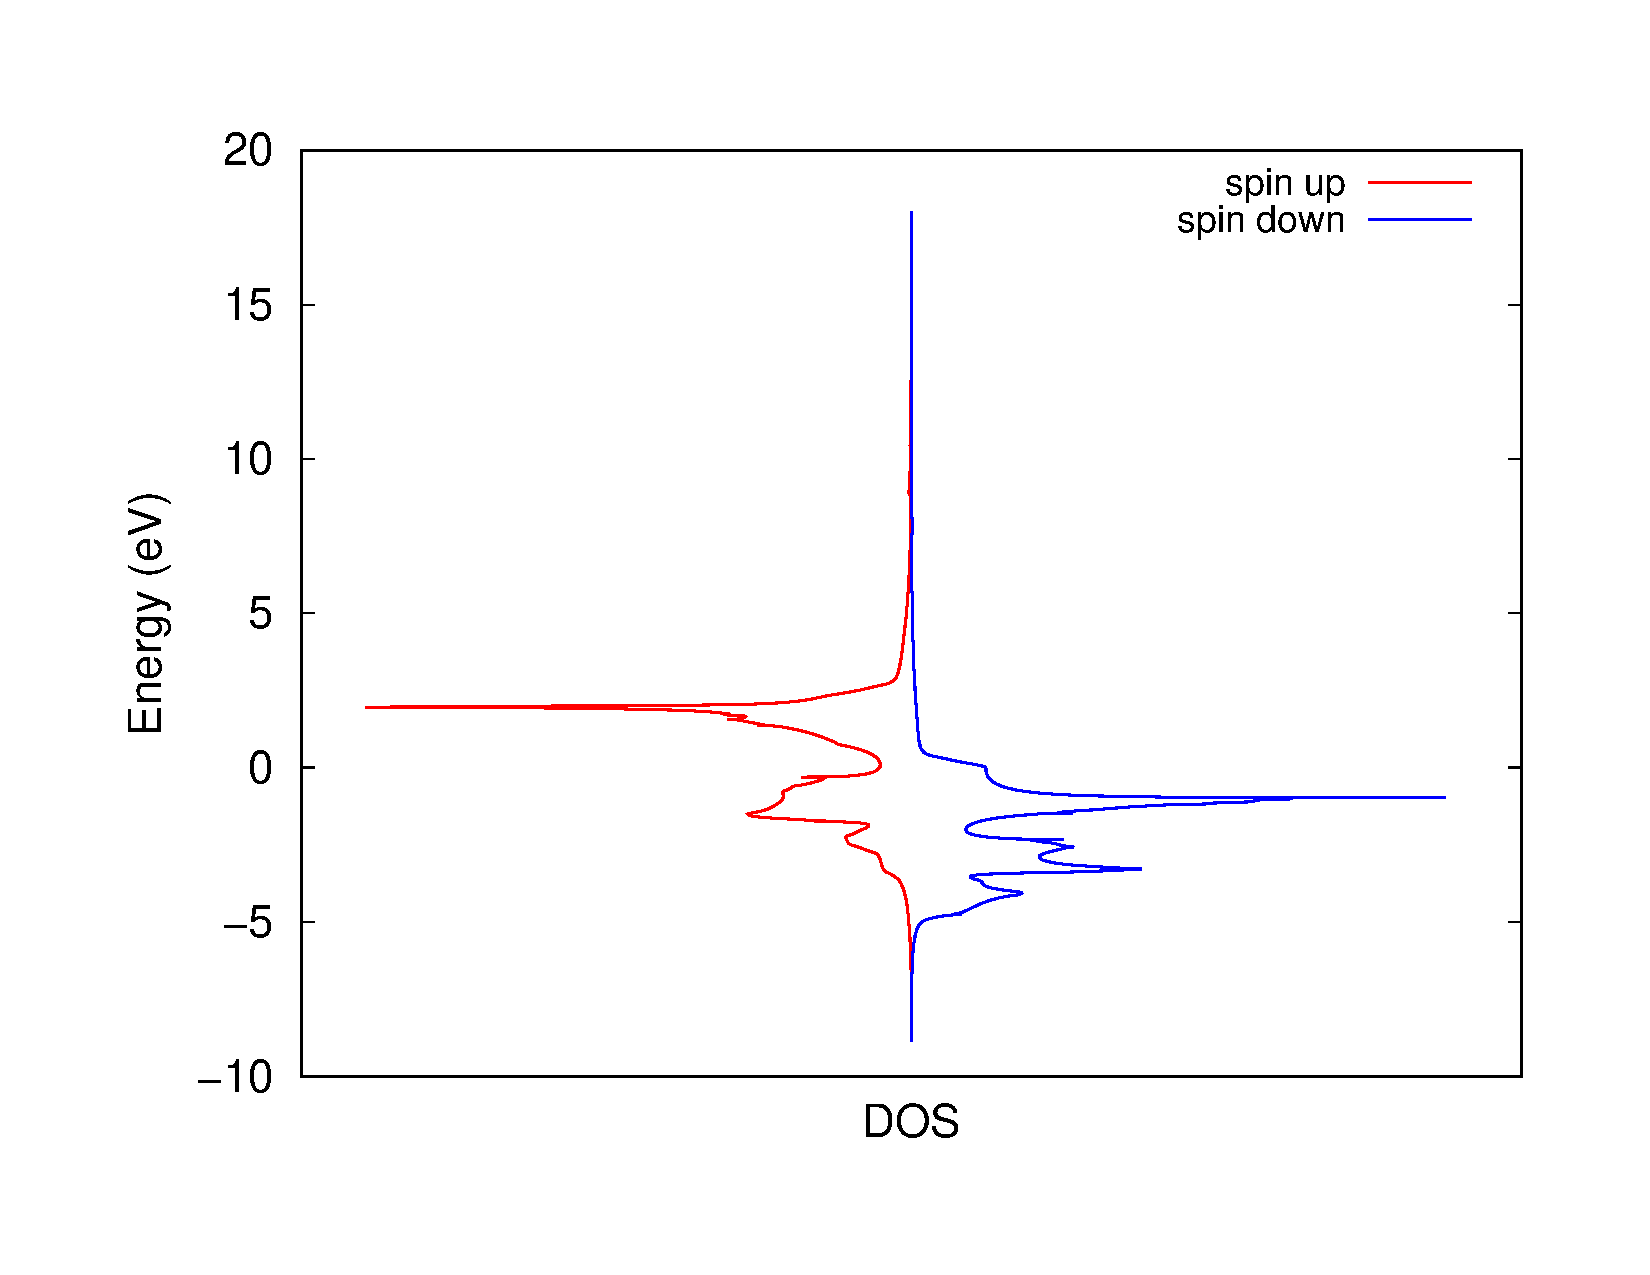
\includegraphics[width=0.7\columnwidth]{figure/example08/DOS_iron_bcc.pdf}
	\caption{Interpolated DOS of bcc iron on a $25\times25\times25$ $\mathbf{k}$-mesh. Up-spin channel (solid red). Down-spin channel (solid blue).}\label{fig8.1}
	\end{figure}
\begin{itemize}
	\item {\it Check the convergence by repeating the DOS calculations with more k-points.}

	Plots of the DOS calculated with different k-point mesh densities for the spin-down channel are shown in \Fig{fig8.2}-(a). In \Fig{fig8.2}-(b)-(c) and (d) we show the convergence of the DOS for the spin-down channel, spin-up channel and both spin channels respectively. The convergence is assessed by looking at the number of states $N$ computed by integrating the DOS up to the Fermi level using the formula
	\begin{equation}
	N_{\uparrow/\downarrow} = \int_{-\infty}^{\epsilon_F}\!\! \mathrm{d}\epsilon\,\, f\tinysub{MV}(\epsilon,\uparrow/\downarrow)\, g(\epsilon,\uparrow/\downarrow), 
	\end{equation}
	where $f\tinysub{MV}(\epsilon,\uparrow) = \int_{-\infty}^{\epsilon} \mathrm{d}\epsilon'\,\widetilde{\delta}(\epsilon')$ is the Marzari-Vanderbilt occupation number function, with $$\widetilde{\delta}(x) = \frac{2}{\sqrt{\pi}}e^{-[x-(1/\sqrt{2})]^2}(2\,-\,\sqrt{2}x), \quad x=\frac{\mu-\epsilon}{\sigma},$$
	where $\epsilon_F$ is the Fermi energy ($12.6256$ eV) and $\sigma$ is the smearing ($0.02$ eV). $g(\epsilon,\uparrow)$ is the DOS from \Wannier{} interpolation. 


	\begin{figure}[h!]
	\centering
	\subfloat[DOS spin $\downarrow$]
	{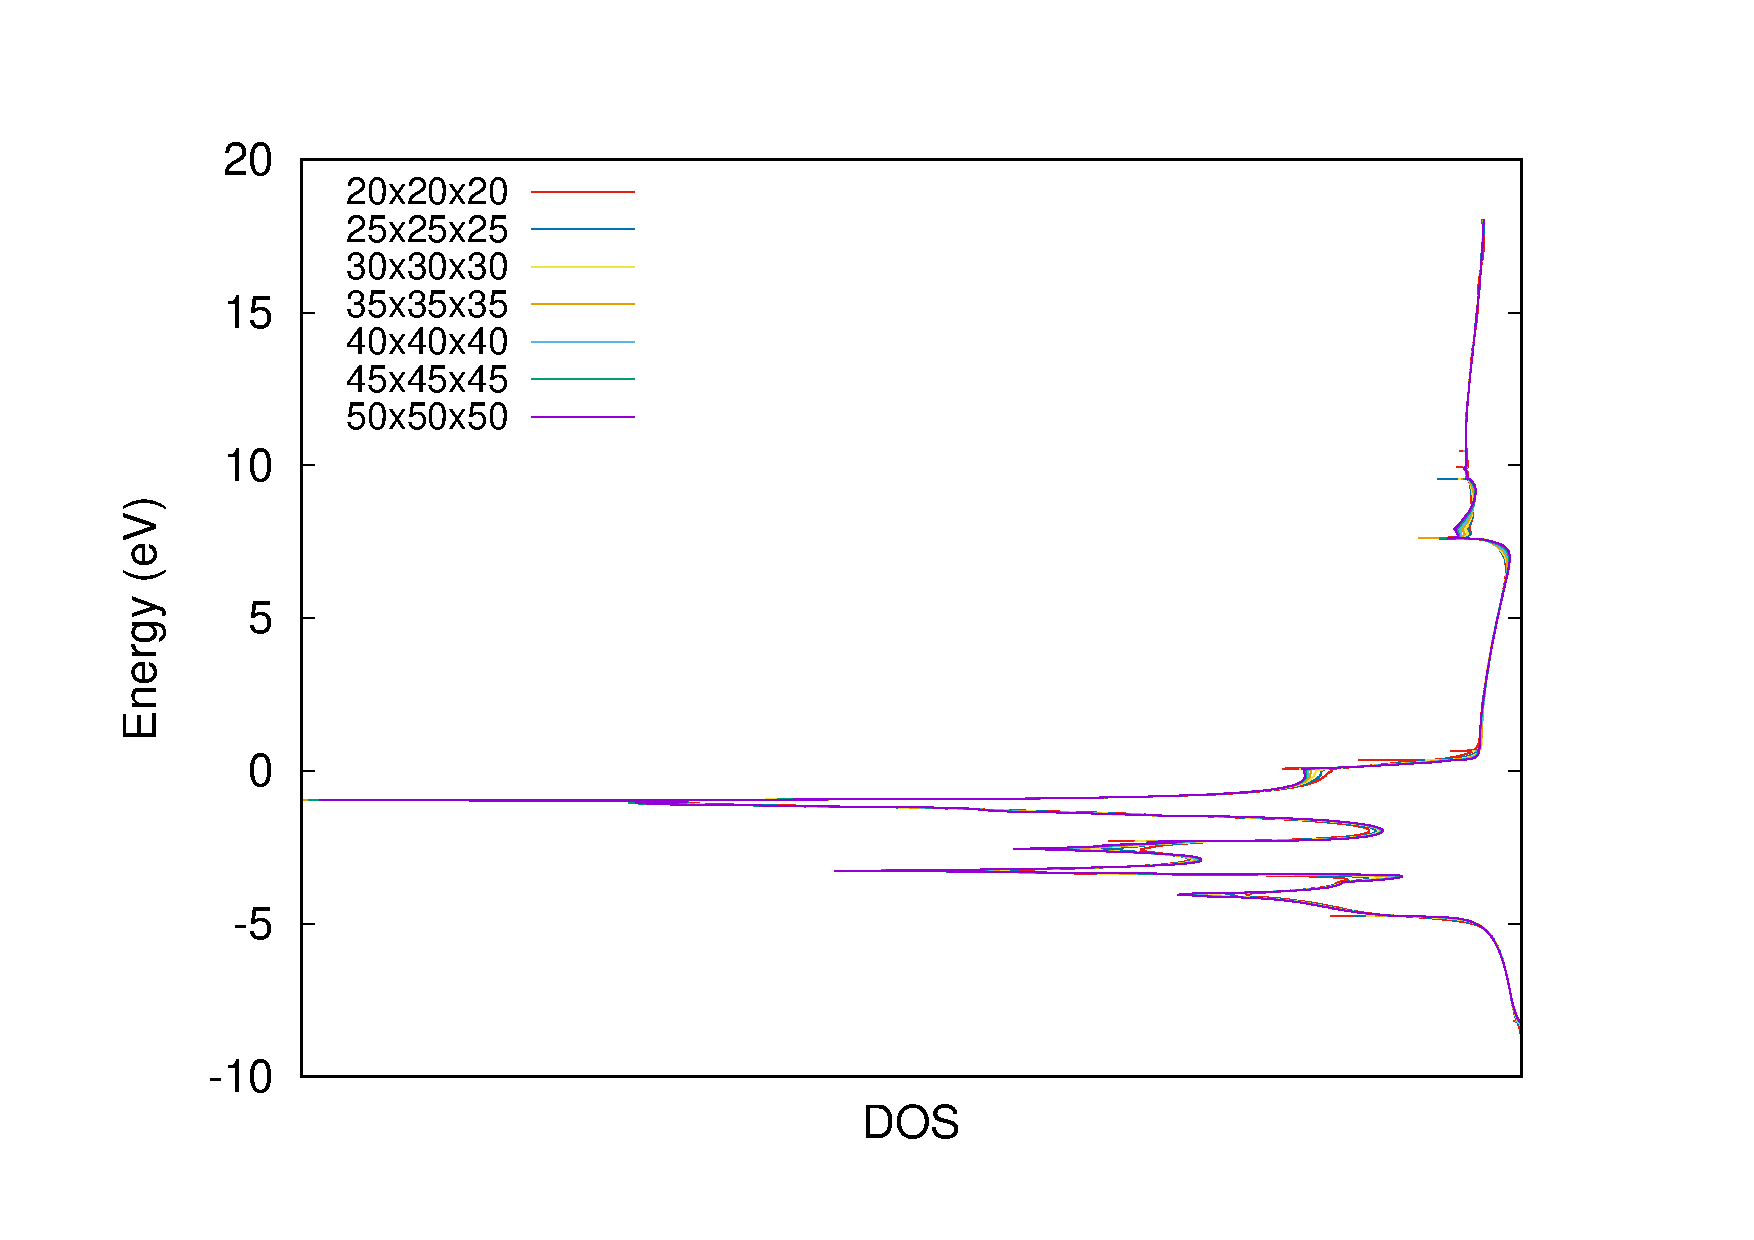
\includegraphics[width=0.5\columnwidth]{figure/example08/DOS_iron_bcc_convergence_down.pdf}}
	\subfloat[$N_\downarrow$]
	{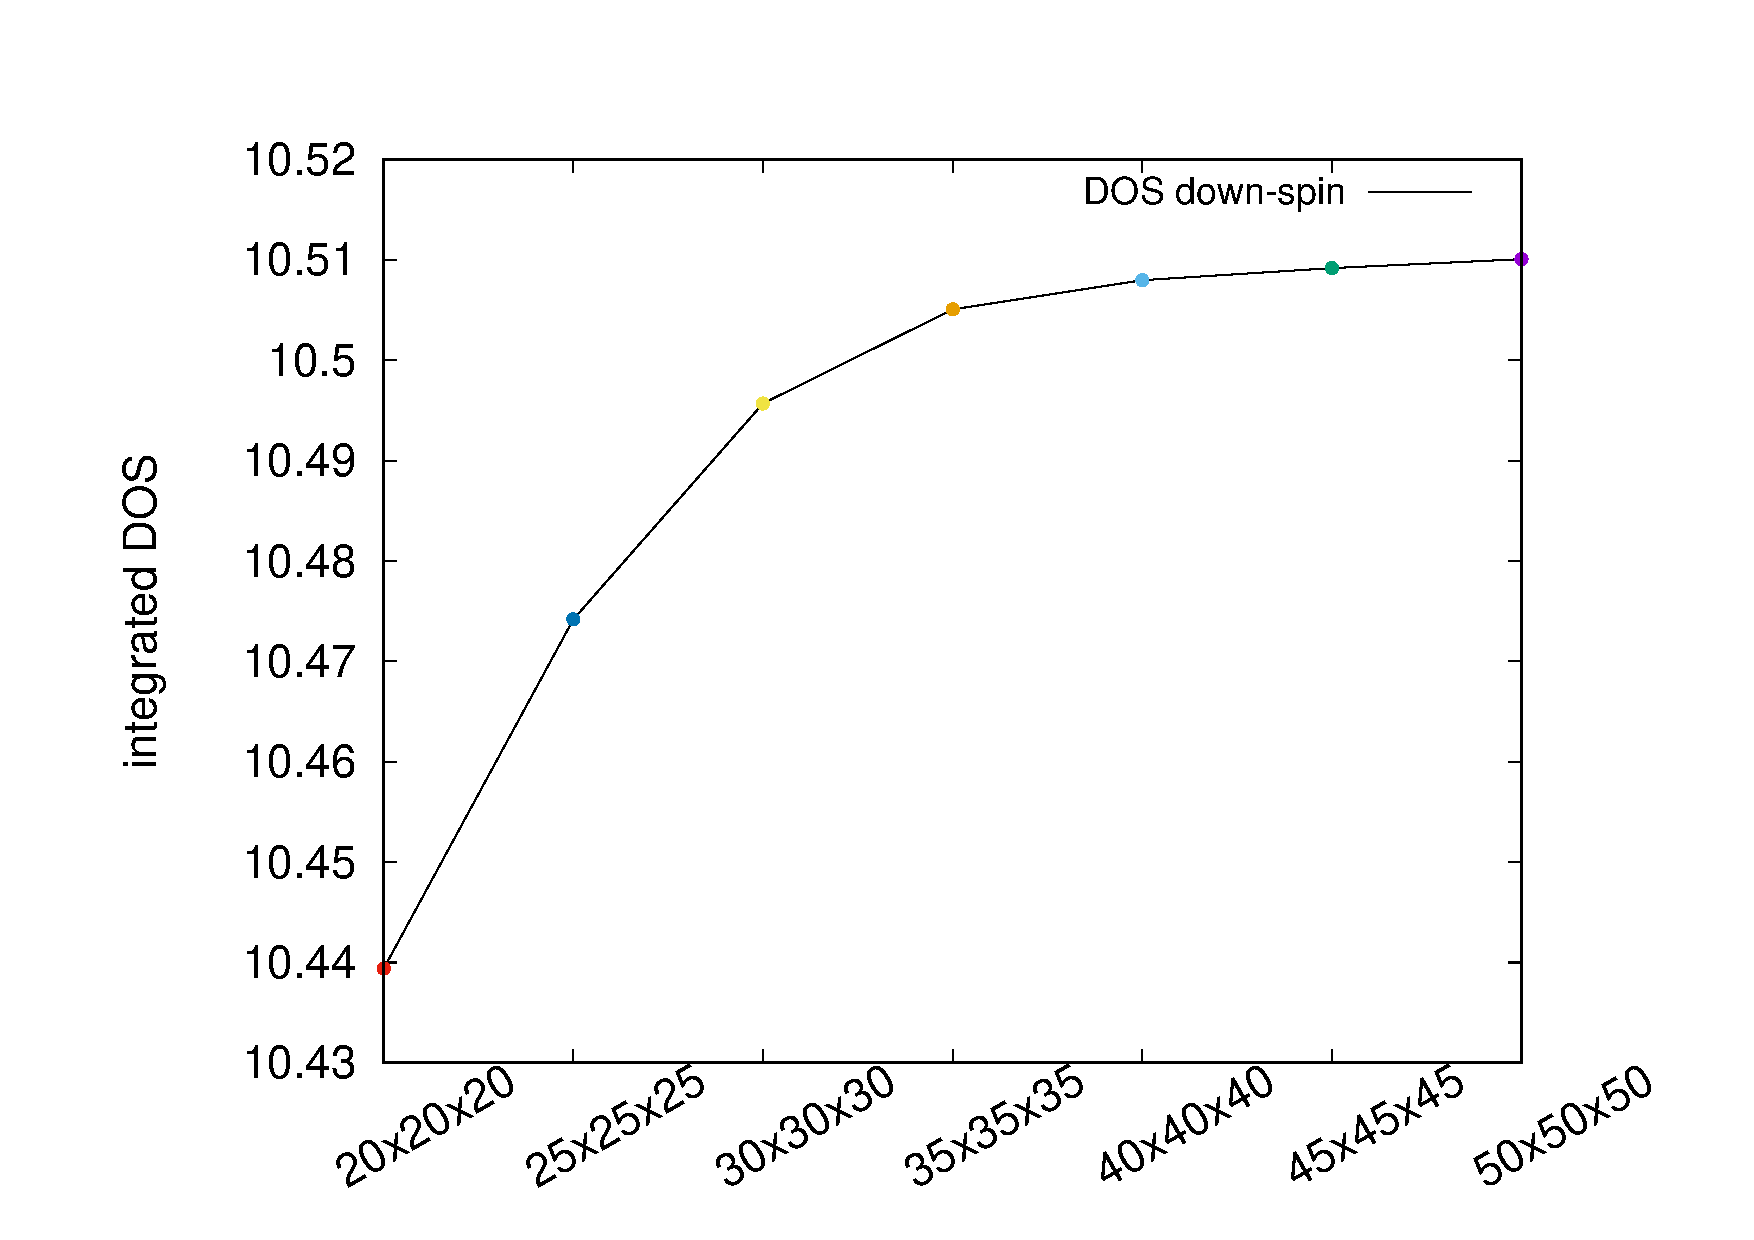
\includegraphics[width=0.5\columnwidth]{figure/example08/convergence_dos_dn_integral.pdf}} \\
	\centering
	\subfloat[$N_\uparrow$]
	{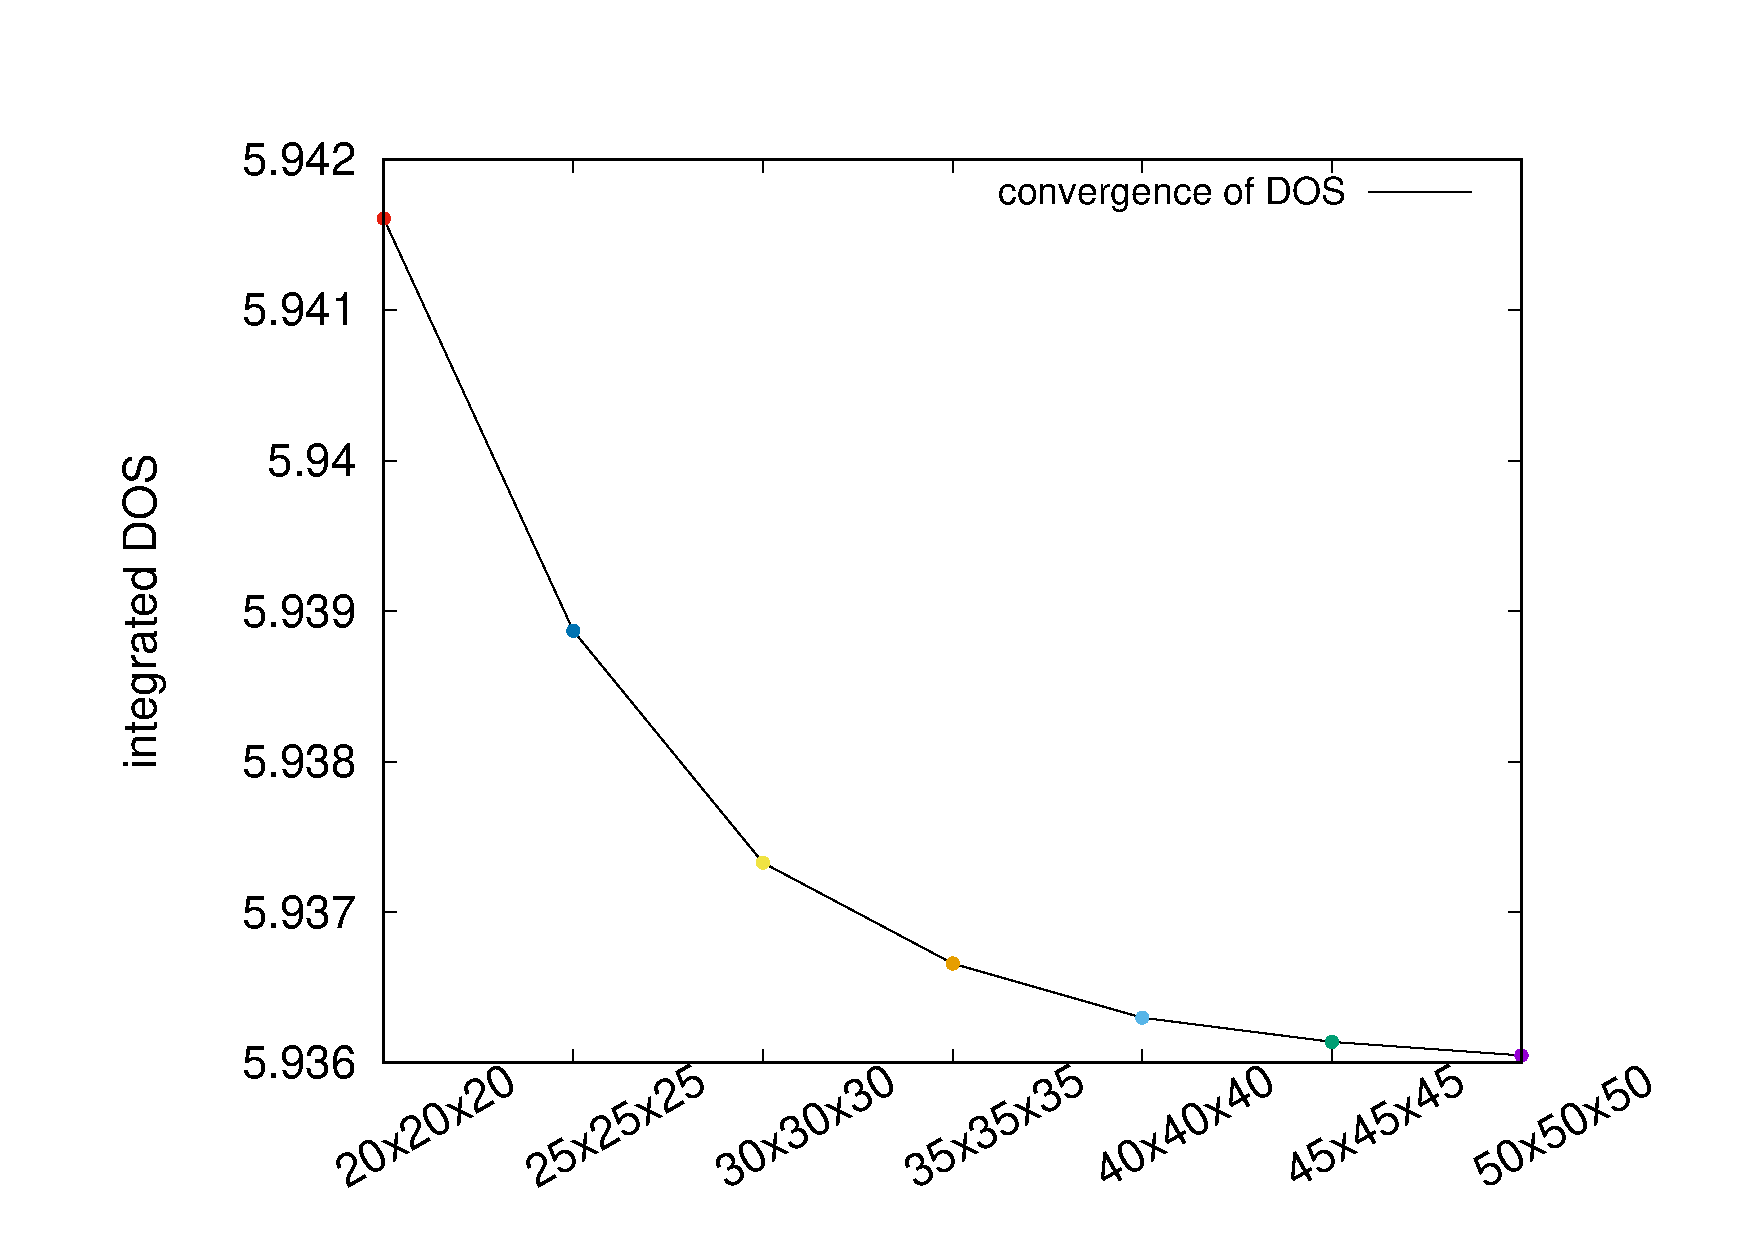
\includegraphics[width=0.5\columnwidth]{figure/example08/convergence_dos_up_integral.pdf}}
	\subfloat[$N_{\uparrow+\downarrow}$]
	{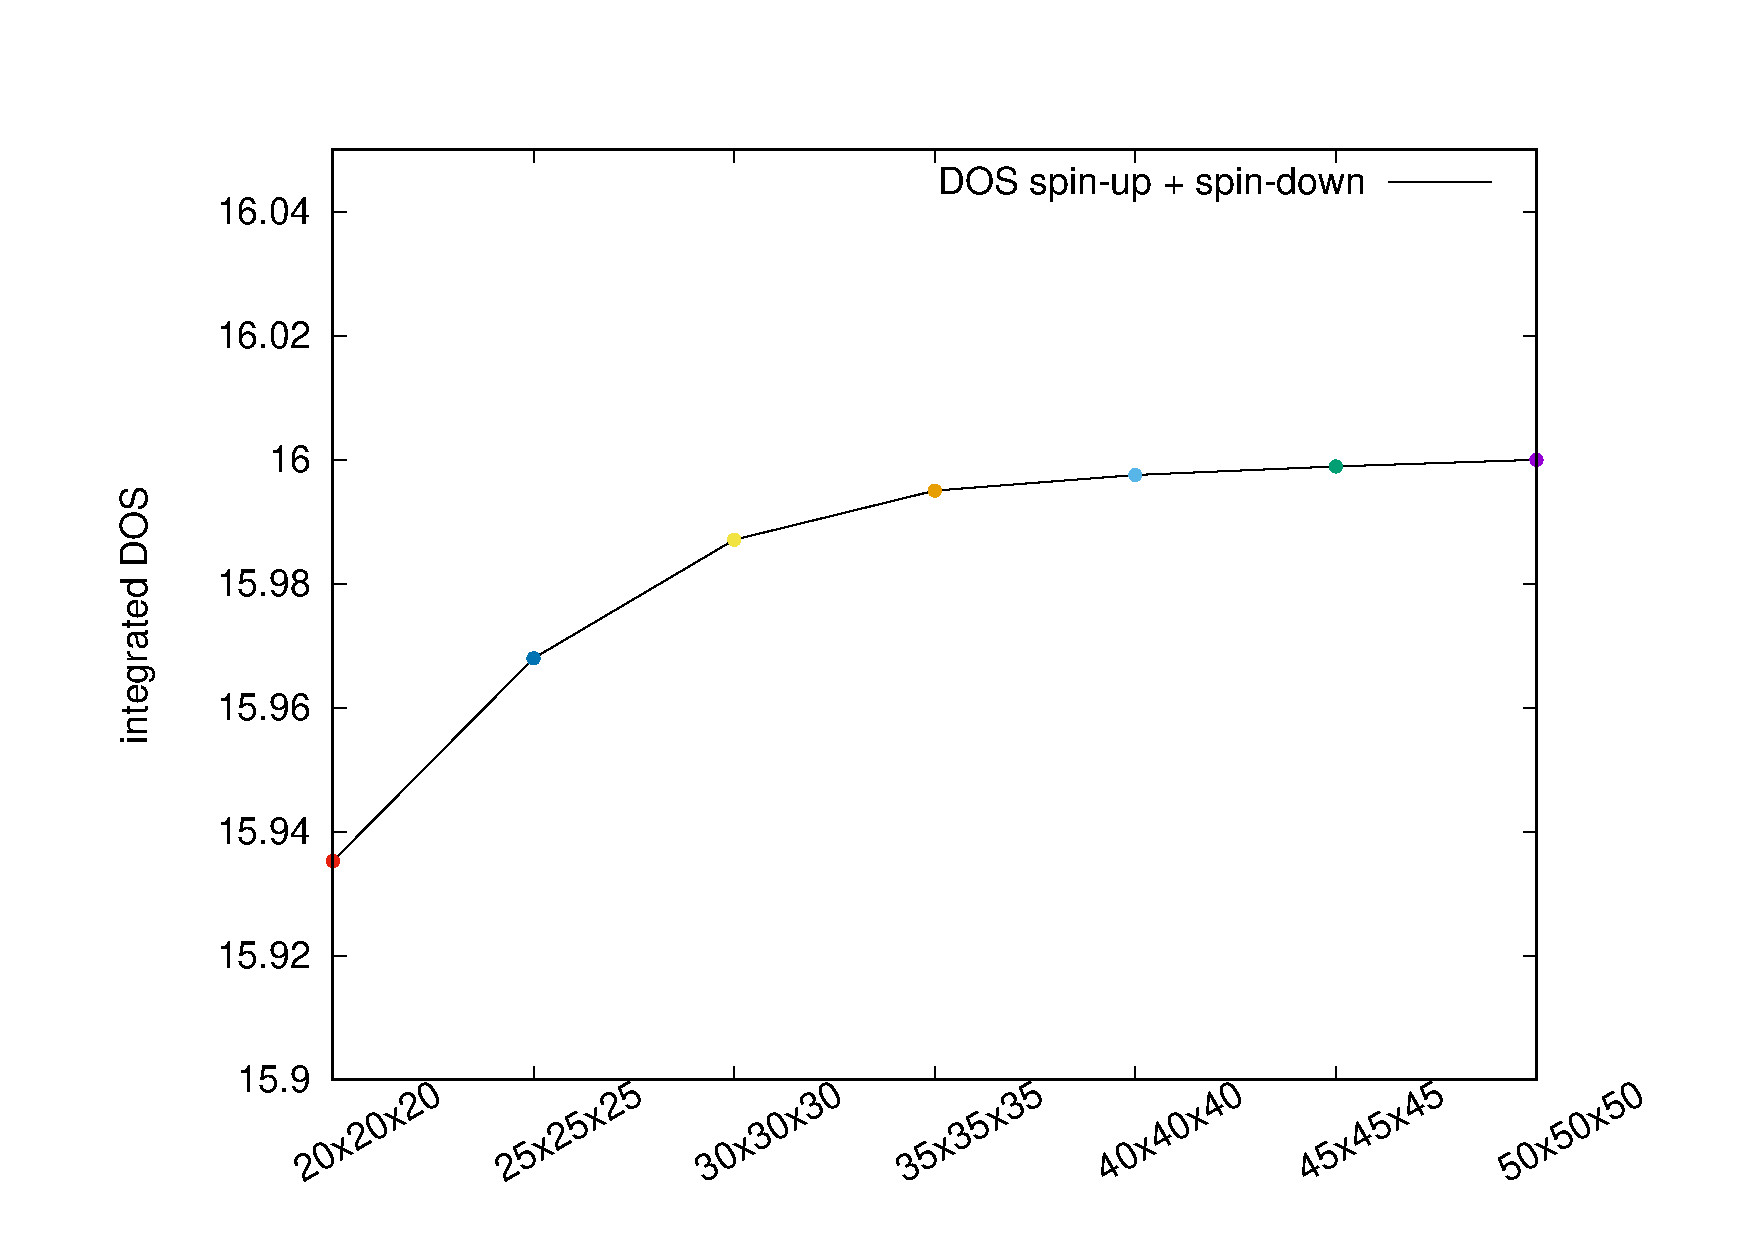
\includegraphics[width=0.5\columnwidth]{figure/example08/convergence_dos_tot_integral.pdf}} 
	\caption{Panel (a) interpolated DOS for the up-spin channel of bcc iron for different $\mathbf{k}$-mesh sizes. Panel (b) corresponding integrated DOS. The integral of the DOS is used as a convergence criterion. $N_{\uparrow+\downarrow}$ has been scaled such as the final value is equal to the total number of electrons.}\label{fig8.2}
	\end{figure}
\end{itemize}
\clearpage
\subsection*{Projected versus maximally-localized Wannier functions}
\begin{itemize}
	\item {\it Open one of the {\tt .wout} files and search for ``Initial state''; those are the projected WFs.} 
	
	For the spin-up channel one finds
	  \begin{tcolorbox}[sharp corners,boxrule=0.5pt]
  {\small
	\begin{verbatim}
	 Initial State
  WF centre and spread    1  ( -0.000000, -0.000000, -0.000000 )     2.25930561
  WF centre and spread    2  ( -0.000000,  0.000000, -0.000000 )     2.32454089 
  WF centre and spread    3  (  0.000000,  0.000000, -0.000000 )     2.32428592 
  WF centre and spread    4  (  0.000000, -0.000000, -0.000000 )     2.32428592 
  WF centre and spread    5  ( -0.000000,  0.000000, -0.000000 )     0.54443303
  WF centre and spread    6  (  0.000000, -0.000000, -0.000000 )     0.51353680
  WF centre and spread    7  (  0.000000,  0.000000, -0.000000 )     0.51353680
  WF centre and spread    8  (  0.000000,  0.000000, -0.000000 )     0.54447716
  WF centre and spread    9  (  0.000000,  0.000000,  0.000000 )     0.51347734 
  Sum of centres and spreads (  0.000000, -0.000000, -0.000000 )    11.86187946
	\end{verbatim}
	}
	\end{tcolorbox}
	It is clear from the spreads and the centres that these are the projected WFs. In particular, WF 1 is the $s$-projected WF. WF 2-4 are the $p$-projected WFs and WF 5-9 are the $d$-projected WF, with $e_g$ (5,8) and $t2_g$ (6,7,9) charachter, respectively (see \Fig{fig8.5}). 
	\begin{figure}[h!]
	\centering
	\subfloat[$s$-type]{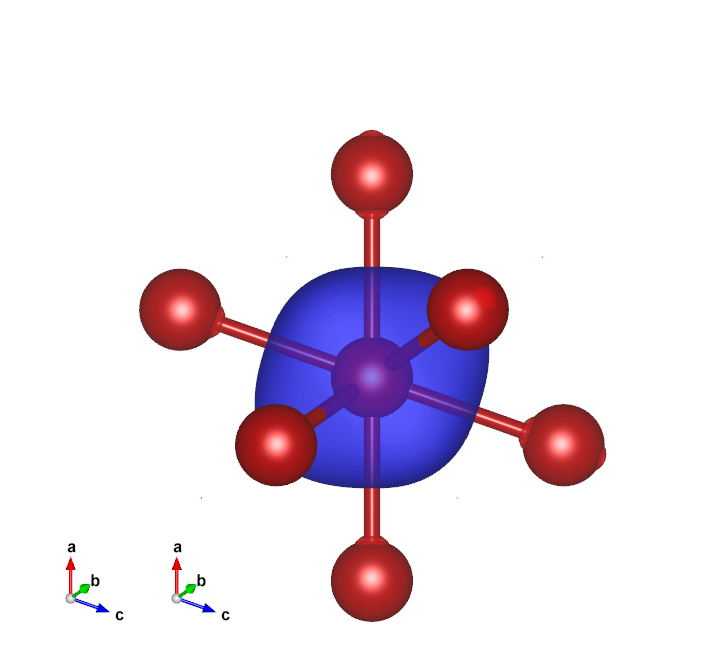
\includegraphics[scale=0.22,trim={130pt 0pt 100pt 70pt},clip]{figure/example08/iron_up_00001_proj.png}}
	\hspace{1.5cm}
	\centering
	\subfloat[$p$-type]{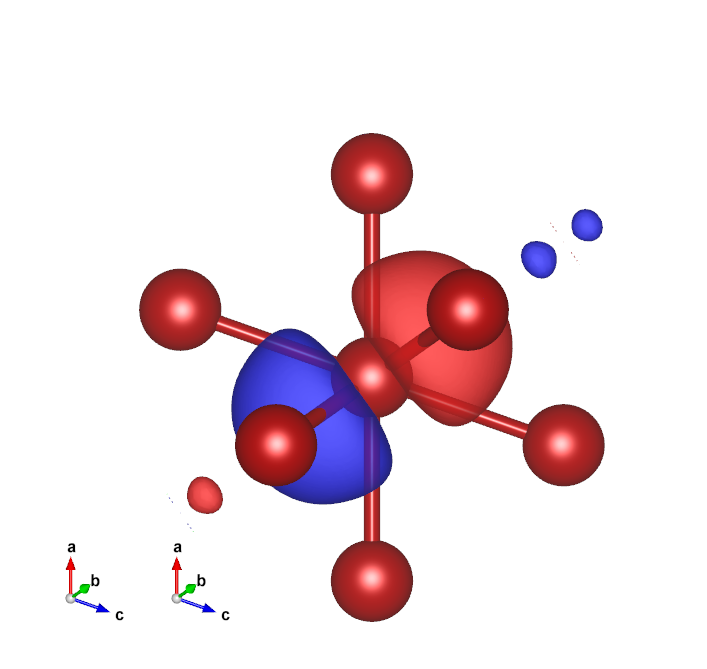
\includegraphics[scale=0.22,trim={130pt 0pt 100pt 70pt},clip]{figure/example08/iron_up_00002_proj.png}}
	\hspace{1.5cm}
	\centering
	\subfloat[$d$-type]{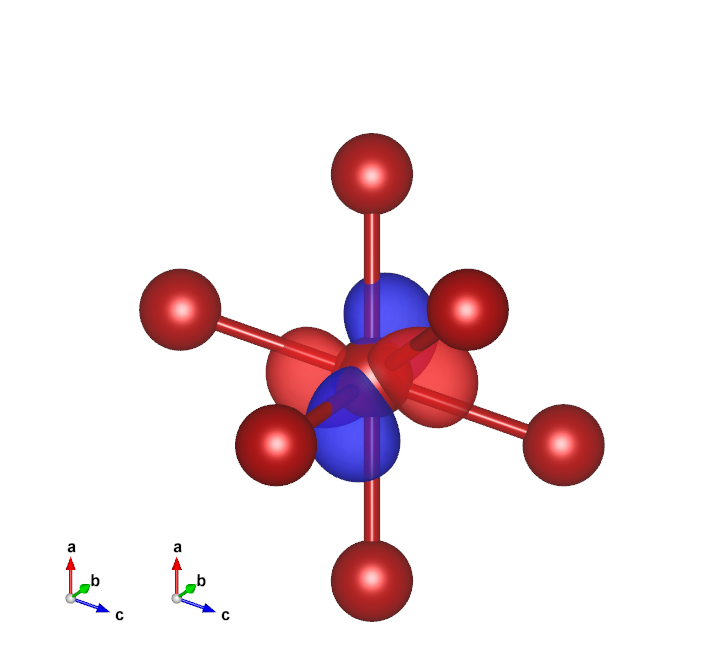
\includegraphics[scale=0.22,trim={130pt 0pt 100pt 70pt},clip]{figure/example08/iron_up_00006_proj.png}}
	\caption{3 representative MLWFs from the wannierisation via projections of 9 spin-up bands of iron. a) MLWF from projection onto 1 $s$ orbital. b) A representative of the MLWFs from projection onto $p$ orbitals. c) A representative of the MLWFs from projection onto $d$ orbitals.}\label{fig8.5}
	\end{figure}


	\item  The Wannier spreads have re-organized in two groups, 6+3; moreover, the six more diffuse WFs are off-centred: the initial atomic-like orbitals hybridized with one another, becoming more localized in the process.
    \newpage
      \begin{tcolorbox}[sharp corners,boxrule=0.5pt]
  {\small
	\begin{verbatim}
	 Final State
  WF centre and spread    1  ( -0.709852,  0.000191,  0.000015 )     1.08935227
  WF centre and spread    2  ( -0.000015, -0.000041, -0.709852 )     1.08935223
  WF centre and spread    3  (  0.709852, -0.000191, -0.000015 )     1.08935227
  WF centre and spread    4  ( -0.000191, -0.709852,  0.000041 )     1.08935226
  WF centre and spread    5  (  0.000015,  0.000041,  0.709852 )     1.08935227
  WF centre and spread    6  ( -0.000000, -0.000000,  0.000000 )     0.43234437
  WF centre and spread    7  (  0.000000,  0.000000,  0.000000 )     0.43234440
  WF centre and spread    8  (  0.000191,  0.709852, -0.000041 )     1.08935228
  WF centre and spread    9  ( -0.000000,  0.000000,  0.000000 )     0.43234438
  Sum of centres and spreads ( -0.000000, -0.000000, -0.000000 )     7.83314672
	\end{verbatim}
	}
	\end{tcolorbox}

	\item {\it The first plateau corresponds to atom-centred WFs of separate s, p, and d character, and the sharp
drop signals the onset of the hybridization. With hindsight, we can redo steps 4 and 5 more efficiently
using trial orbitals with the same character as the final MLWFs,
{\tt

Fe : sp3d2;dxy;dxz;dyz

}}
With this choice the minimization converges much more rapidly as can be seen in Fig.~\ref{fig8.4}-(a).
\item {\it Let us recompute the DOS using, instead of MLWFs, the WFs obtained by projecting onto s, p, and d-type trial orbitals.}
\begin{figure}[h!]
\centering
\subfloat[]{
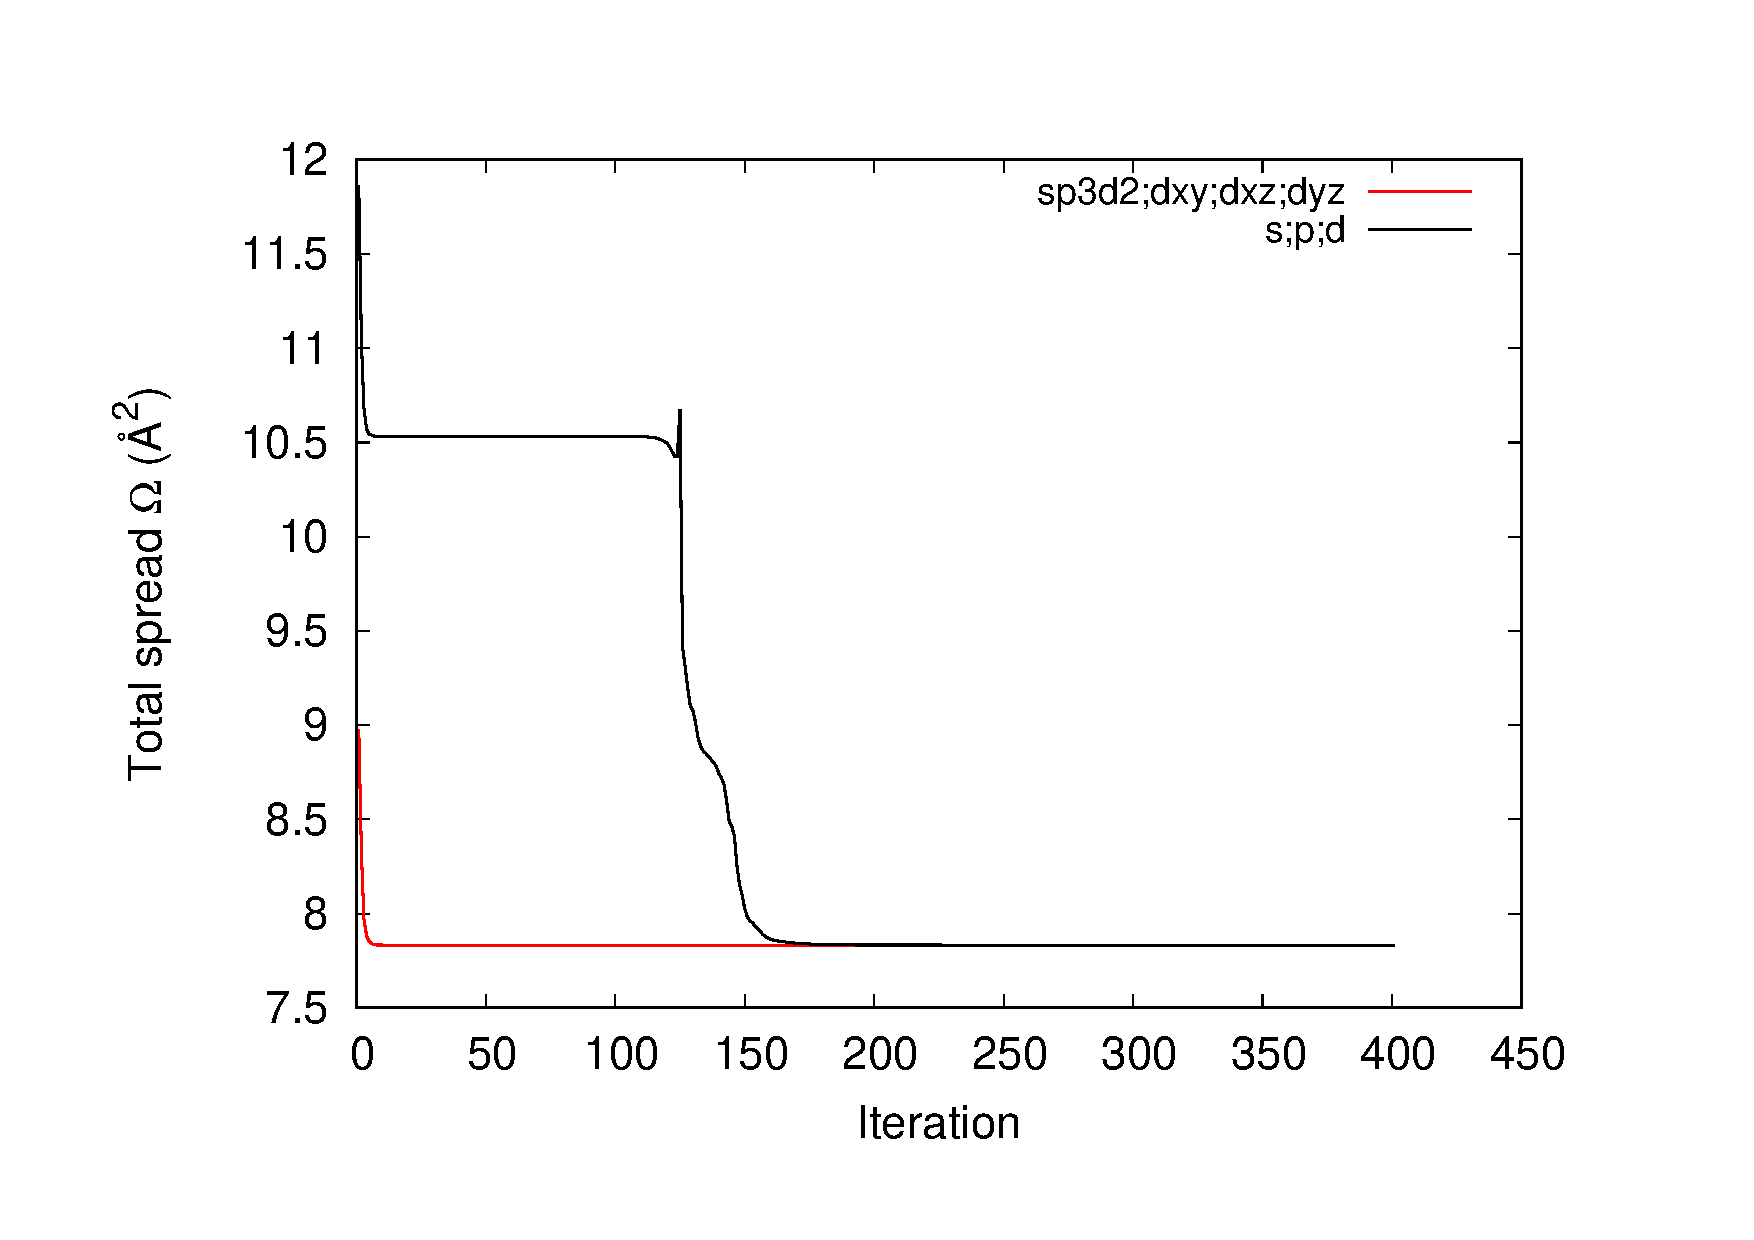
\includegraphics[width=0.45\columnwidth,trim={50pt 40pt 50pt 50pt},clip]{figure/example08/iron_bcc_fast_convergence.pdf}}
\centering
\subfloat[]{
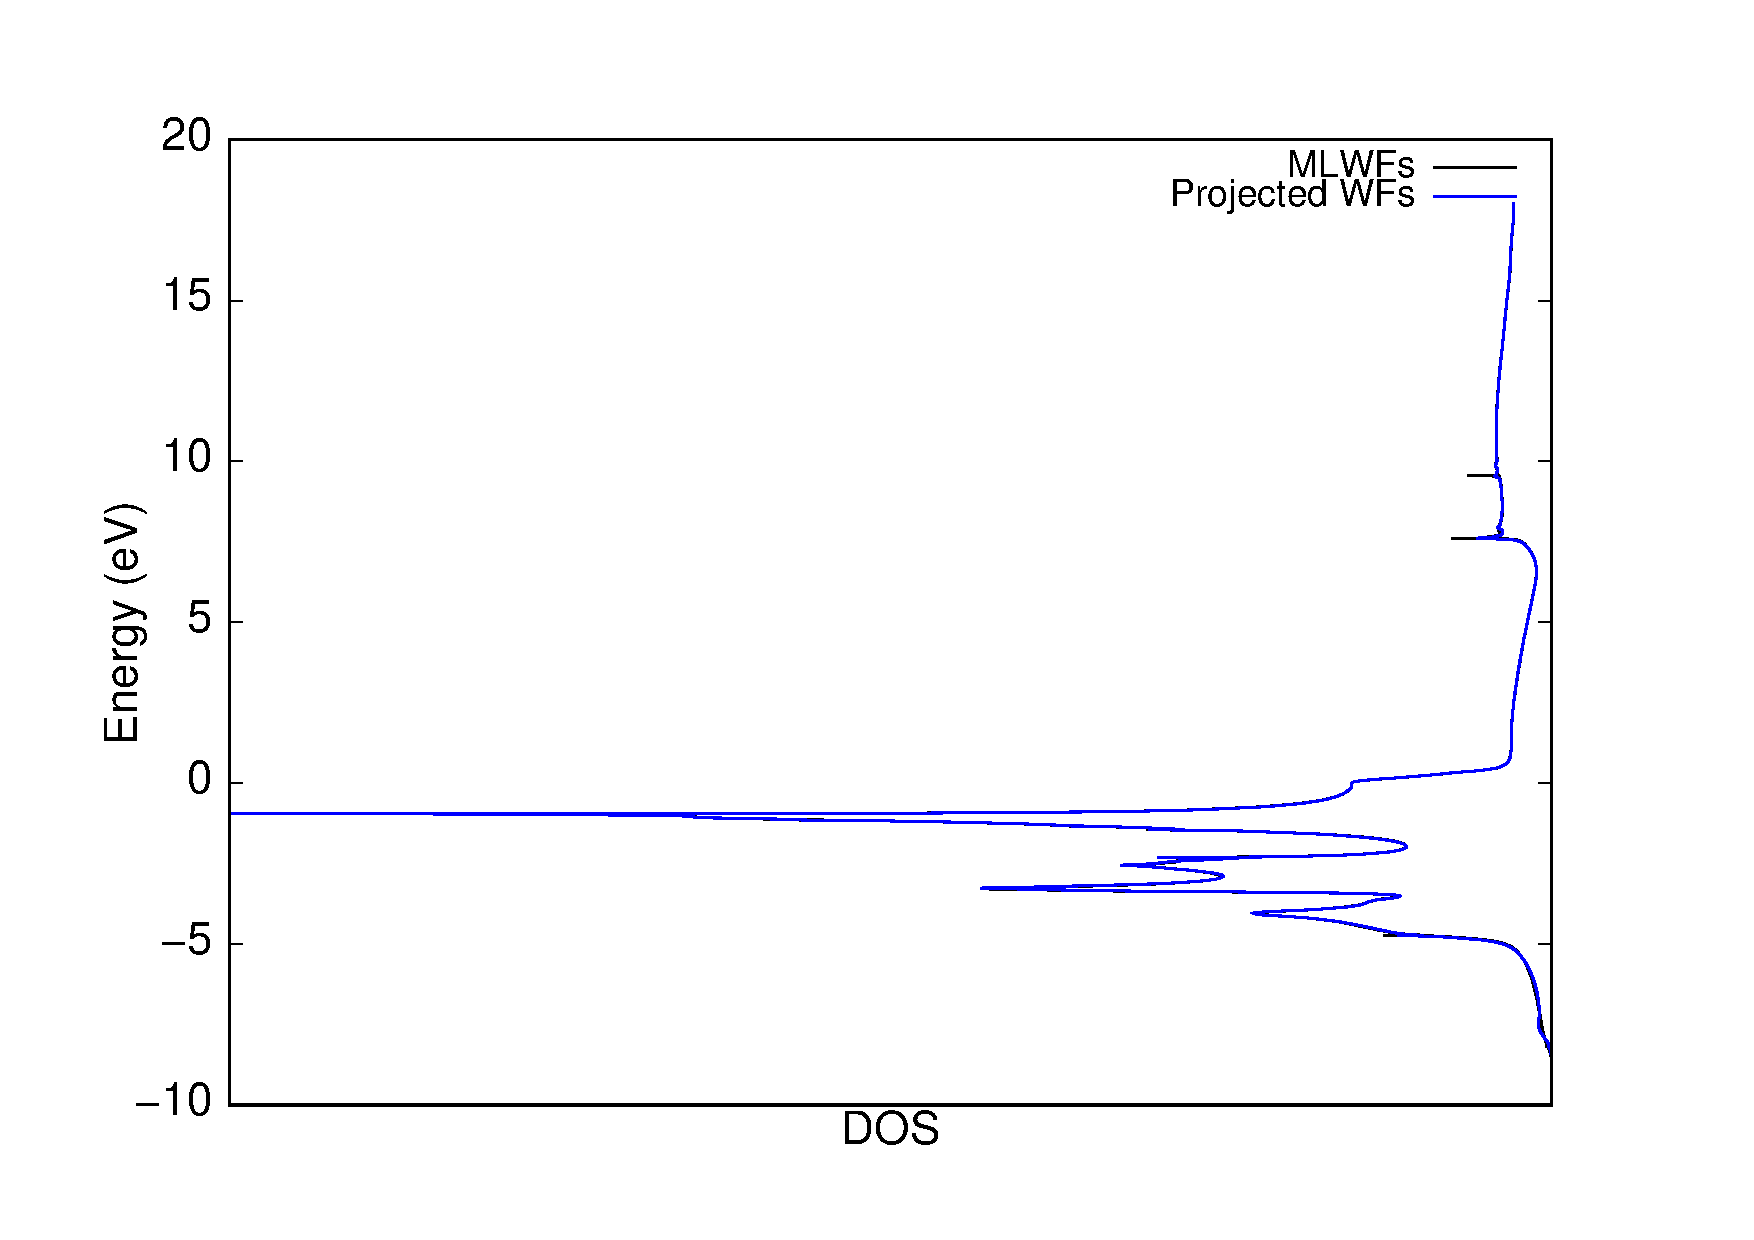
\includegraphics[width=0.45\columnwidth,trim={20pt 20pt 10pt 30pt},clip]{figure/example08/Projected_vs_MLWFs_DOS.pdf}}
\caption{a) Convergence of $\Omega$ for two different sets of initial projections: $s;p;d$ (solid black) and $sp_3d_2;d_{xy};d_{xz};d_{yz}$ (solid red). b) DOS with MLWFs (solid black) and projected $s;p;d$ Wannier functions (solid blue).}\label{fig8.4}
\end{figure}
\end{itemize}

\newpage
\subsection*{Orbital--projected DOS and exchange splitting}
{\it In order to obtain the partial DOS projected onto the $p$--type WFs, add to the {\tt .win} files
{\tt

dos\_project = 2,3,4

}
and re-run {\tt postw90}.} 
\begin{itemize}
\item {\it Plot the projected DOS for both up-- and down--spin bands. Repeat for the $s$ and $d$ projections.}

Results are shown in figure below (\Fig{fig8.7}).

\begin{figure}[h!]
\centering
\subfloat[$s$]{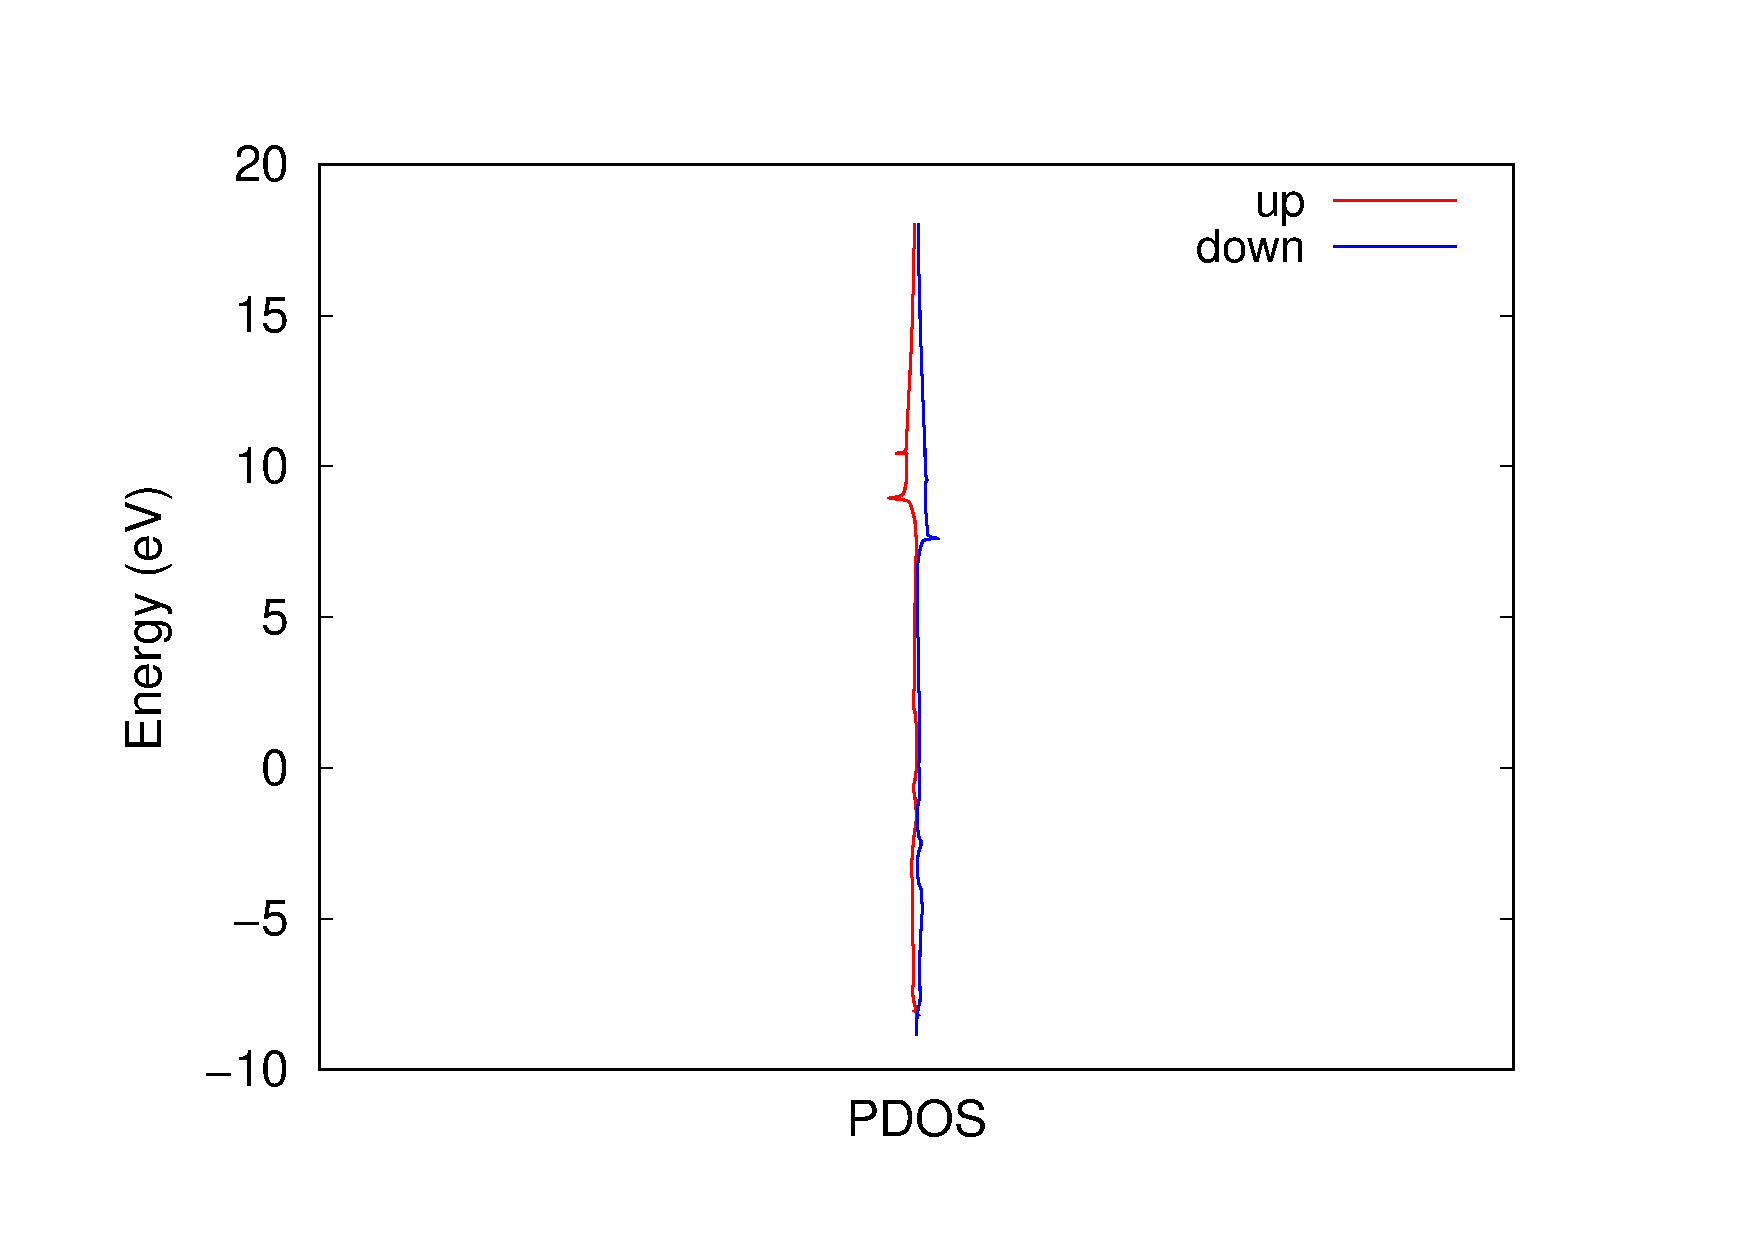
\includegraphics[width=0.33\columnwidth,trim={30pt 30pt 50pt 40pt},clip]{figure/example08/PDOS_updn-spin_s.pdf}}
\centering
\subfloat[$p$]{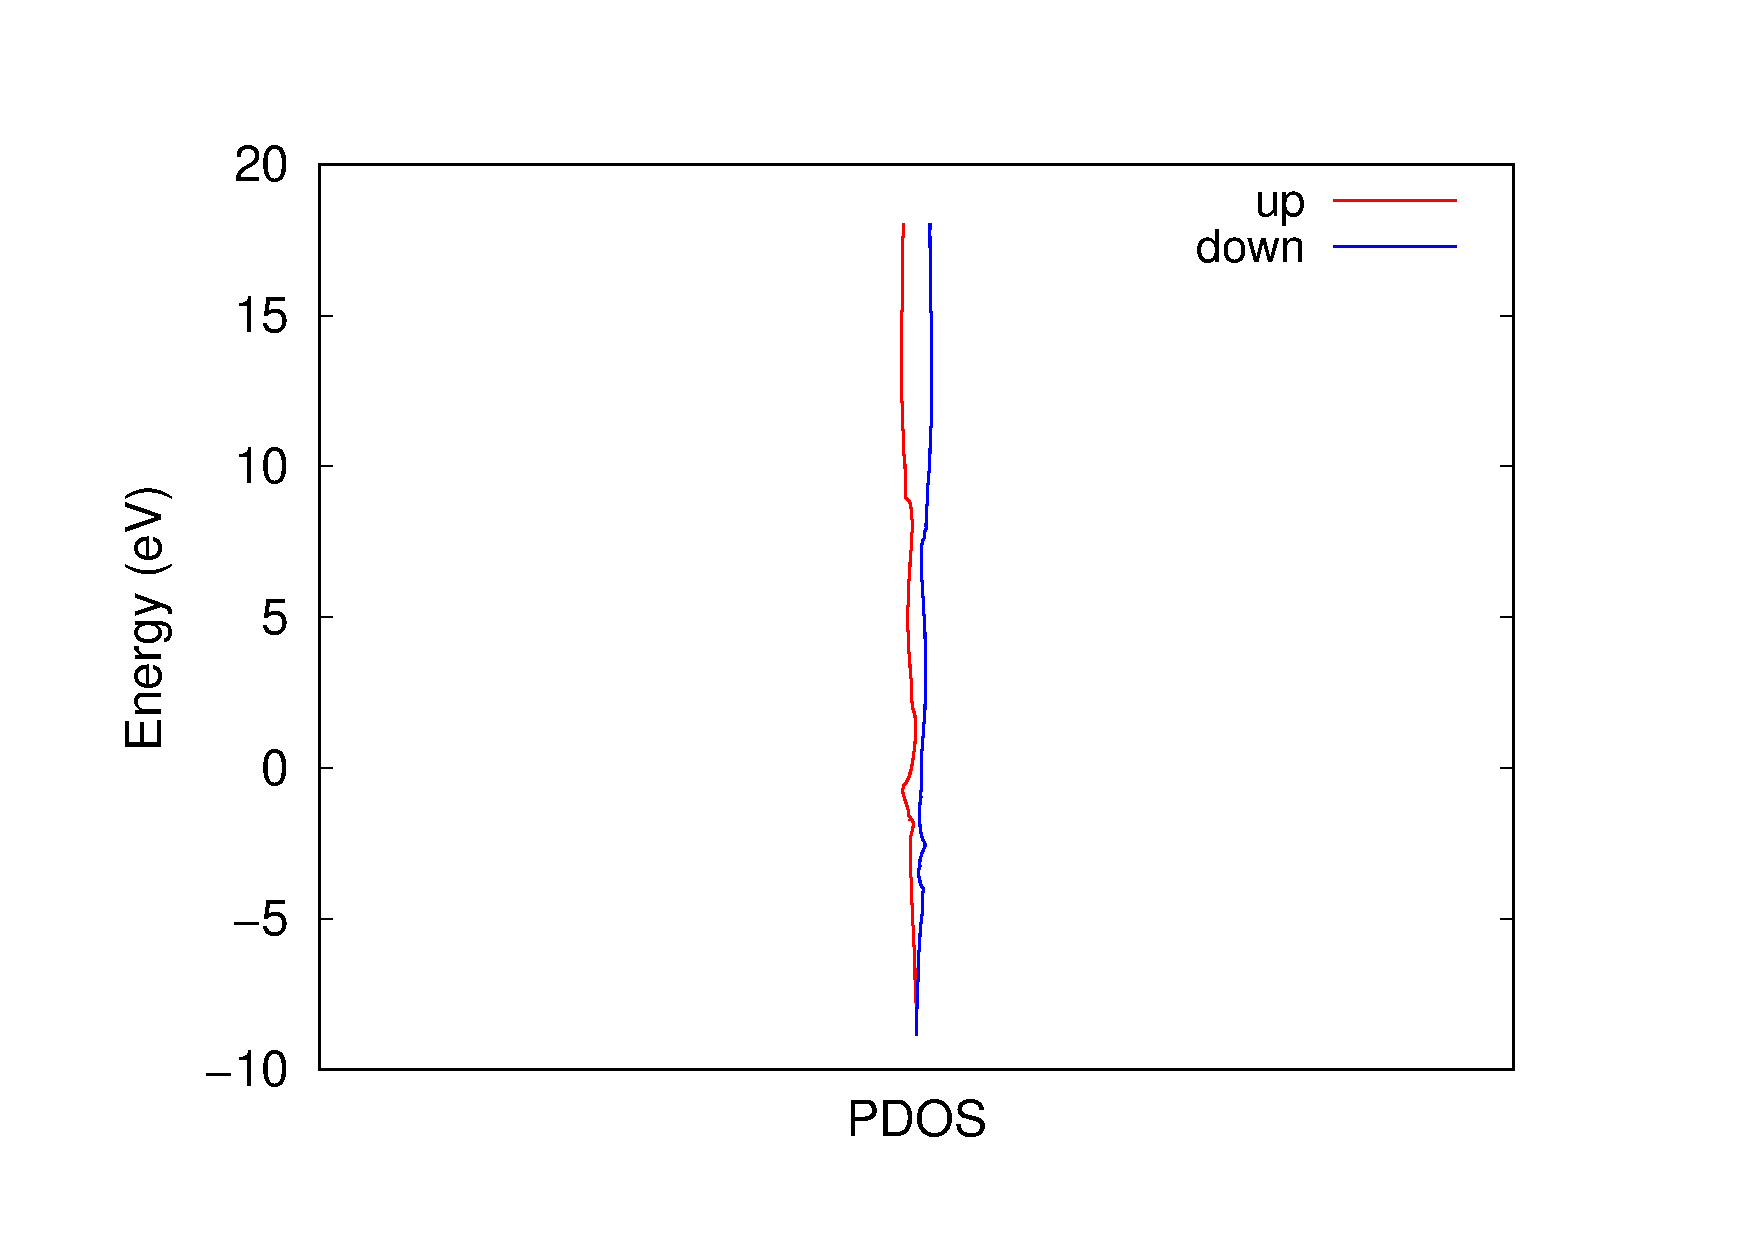
\includegraphics[width=0.33\columnwidth,trim={30pt 30pt 50pt 40pt},clip]{figure/example08/PDOS_updn-spin_p.pdf}}
\centering
\subfloat[$d$]{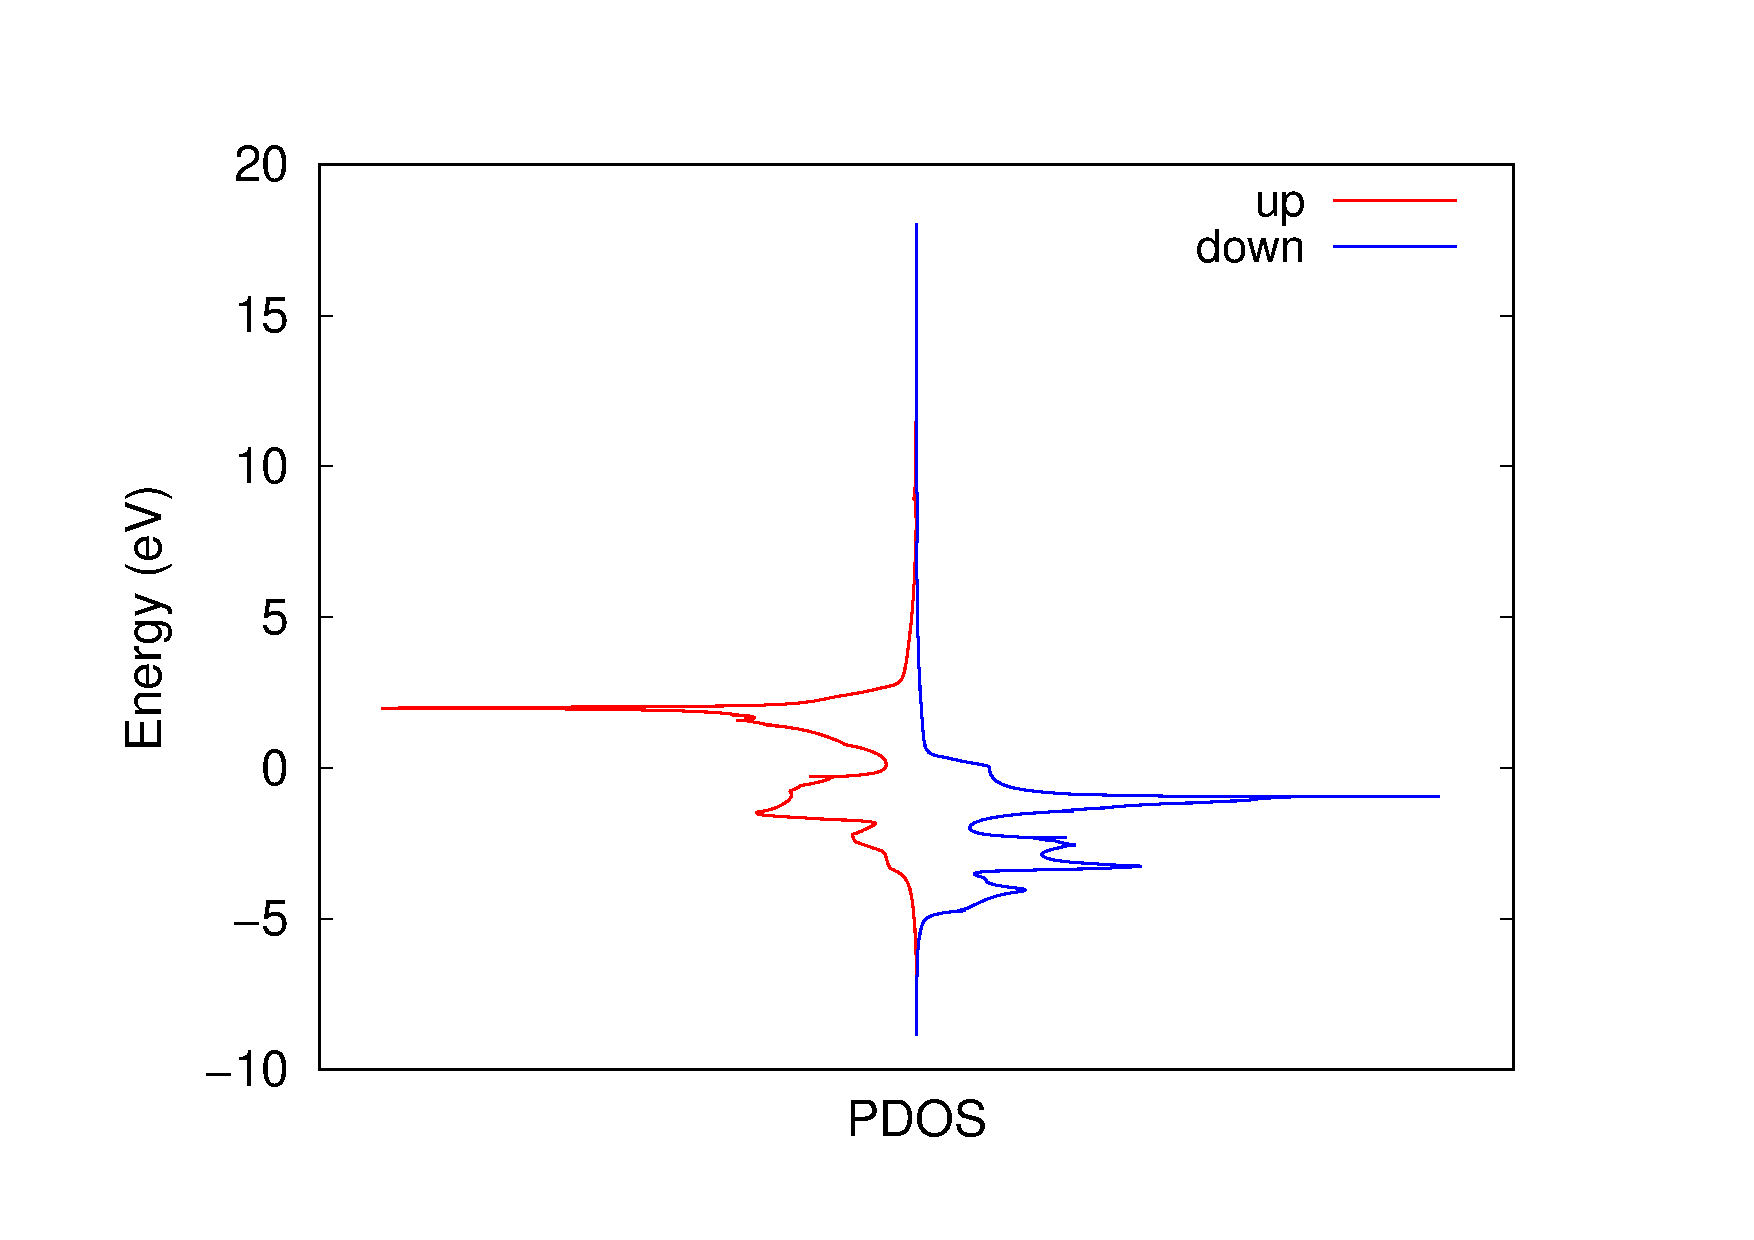
\includegraphics[width=0.33\columnwidth,trim={30pt 30pt 50pt 40pt},clip]{figure/example08/PDOS_updn-spin_d.pdf}}
\caption{Partial DOS projected onto a) 1 $s$-like WF, b) 3$p$-like WFs and c) 5$d$-like WFs.}\label{fig8.7}
\end{figure}


\item {\it The difference between corresponding values of the on-site energies the on-site energies $\braket{\boldsymbol{0}n\vert H \vert \boldsymbol{0}n}$ in {\tt iron\_up.wout} and in {\tt iron\_dn.wout} gives the exchange splittings for the individual orbitals.}

Results are shown in \Tab{tab8.2}. 

 \begin{table}[h!]
 \centering
	\captionsetup{width=.5\textwidth}
	\caption{Exchange splittings for individual orbitals in eV.}
 \begin{tabular}{@{} lcccc @{}}\toprule[1.5pt]
     n &  character &    $\braket{\boldsymbol{0}n\vert H \vert \boldsymbol{0}n}$ for $\downarrow$ & $\braket{\boldsymbol{0}n \vert H \vert \boldsymbol{0}n}$ for $\uparrow$ & $\Delta$ \\
      & & [eV] & [eV] & [eV] \\\midrule
     1 &    $s$ &   21.307132  & 22.074648 & 0.767516 \\
     2 &    $p$ & 26.353088  & 26.817526 & 0.464438 \\
     3 &    $p$ &  26.352956  & 26.817207 & 0.464251 \\
     4 &    $p$ &  26.352956  & 26.817207 & 0.464251 \\
     5 &    $d$ &  10.531720  & 13.206631 & 2.67491 \\
     6 &    $d$ &   10.775917  & 12.808277 & 2.03236 \\
     7 &    $d$ &   10.775917  & 12.808277 & 2.03236 \\
     8 &    $d$ &   10.532108  & 13.207139 & 2.67503 \\
     9 &    $d$ &   10.775177  & 12.807388 & 2.03221  \\\bottomrule[1pt]
\end{tabular}\label{tab8.2}
\end{table}


\item Compare their magnitudes with the splittings displayed by the orbital-projected DOS plots


\end{itemize}
